The followed informations introduce the results in two cases. 
In the first, the algorithm makes the tracking of an object with 
a displacement perpendicular to the observer (approximately 2D displacement),
giving us informations about its relative position. 
In the second, the program detects the approach of target and 
slight movement in axis x and y.


The next images, available by KITTI, are used to test in 2D. 
The initial position is in the image (a) and final position in (b), 
so it is generated a vector that begin in the initial point and final 
point to illustrate the track made.

\begin{figure}[H]
\centering
  \subfloat[]{\label{fig:imgpapercertaa} \includegraphics[width=.5\columnwidth]{images/images/0000000000.png}}
  \subfloat[]{\label{fig:imgpapercertab} \includegraphics[width=.5\columnwidth]{images/images/img_paper_certa.eps}}
  \caption{The image in (a) represents the target in its position 
  initial and the image (b) demonstrates the vehicle in final position with vector 
  that describe its path.}
\end{figure}


We can observe that there is a small bend in the image which 
reflect in the description of algorithm. 
The graphic is not a straight line because the image is curved and,
consequently, there is an impression of approaching. The difference among initial 
and final values may be considered small once they are close.


\begin{figure}[H]
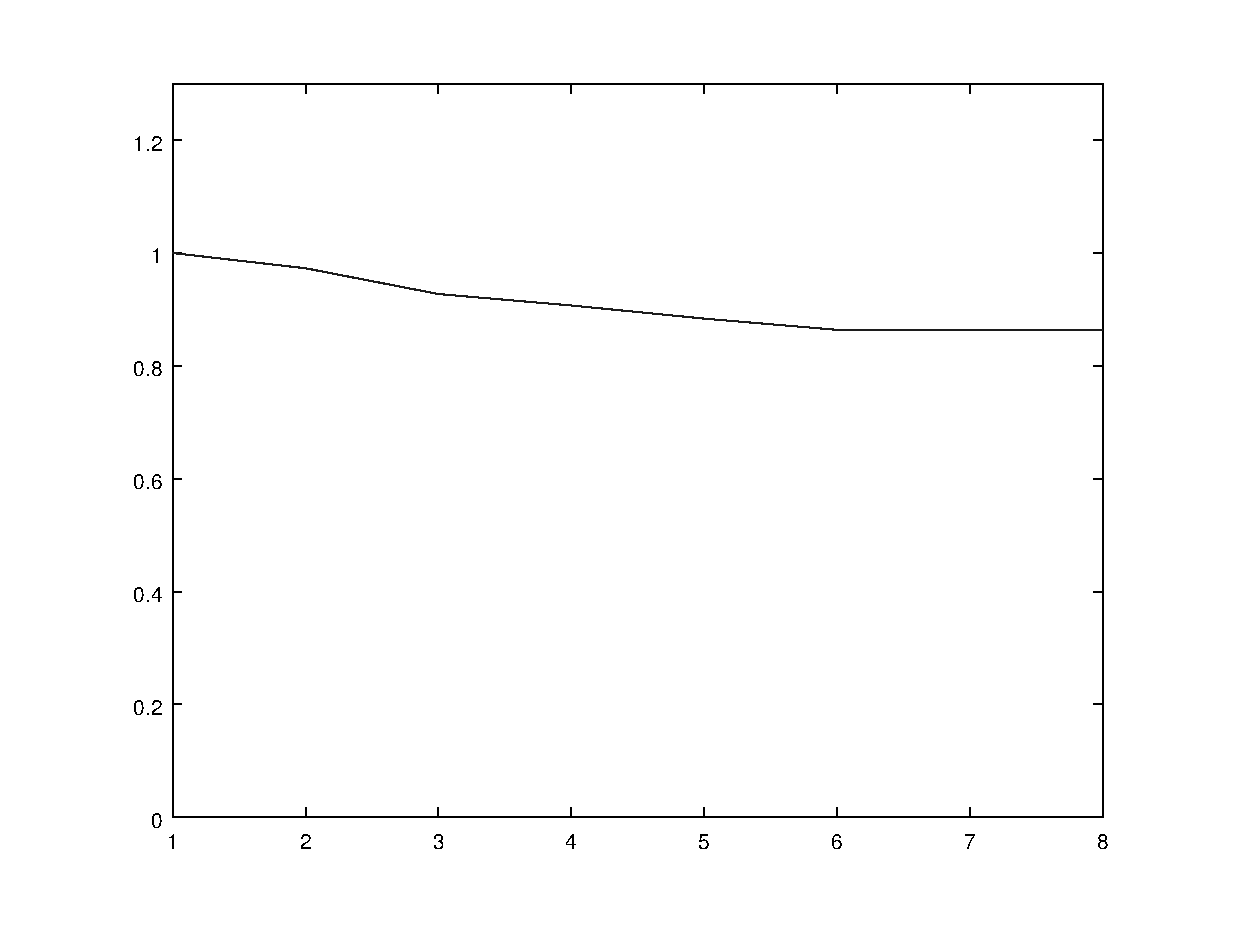
\includegraphics[width=\columnwidth]{images/graph1.eps}
\caption{In this graphic, axis x is frame compared with ROI and axis 
y is factor of approaching or departure.
The curve generated describes an approaching however it is not visible. 
This is happen because images used have a slight curvature.}
\label{fig:res_graph1}
\end{figure}

Although the images have its peculiar characteristics, the program made 
the tracking and generated results that describe exactly the path of 
object, proving the high sensibility of algorithm.

In the second test, we introduce the functionality of algorithm in 3D. 
The program compares the images and calculate the factor of approaching or 
departure based on the area of object. The next figure demonstrates the 
initial and final position of target.

\begin{figure}[H]
\centering
  \subfloat[]{\label{fig:targeinit} \includegraphics[width=.5\columnwidth]{images/images/351.jpg}}
  \subfloat[]{\label{fig:targeend} \includegraphics[width=.5\columnwidth]{images/images/450.jpg}}
  \caption{The object in (a) is the initial position and its area is 
  fewer than the figure in (b), which is in final position. 
  The factor is calculate dividing both areas.}
\end{figure}

The graphic that describes the movement of object is showed in the next figure. 
We can observe the significant increase in area of vehicle. So, it 
contributes, directly, with factor of approaching.

\begin{figure}[H]
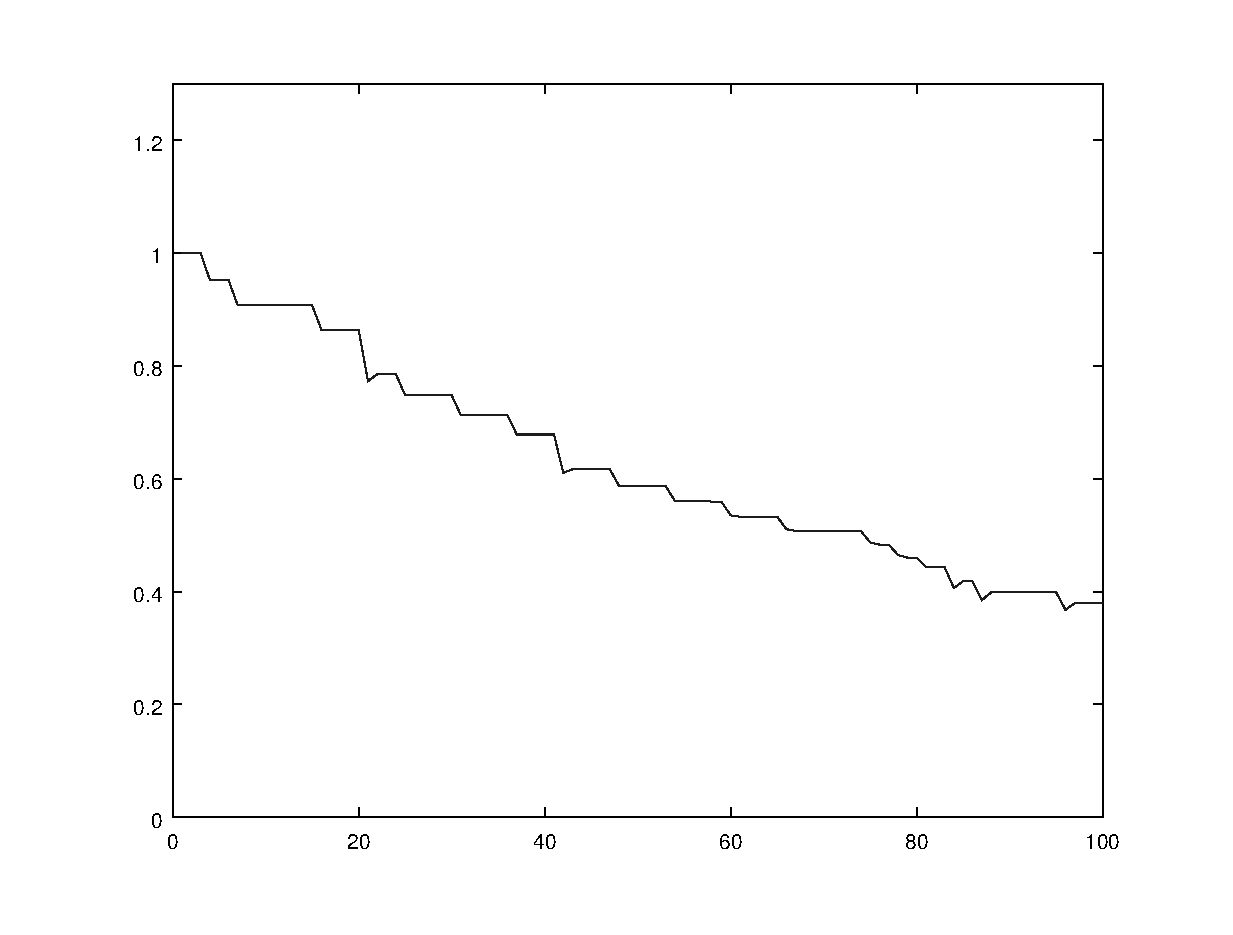
\includegraphics[width=\columnwidth]{images/graph2.eps}
\caption{In this graphic, axis x is frame compared with ROI and axis y is 
factor of approaching or departure.
The curve generated describes an approaching of vehicle. 
Its initial position is given value 1 and all other positions are related to 1.}
\label{fig:res_graph2}
\end{figure}

The graphic of factor per frames could be seen how position per time, 
because the factor describes the position relative target and the amount of 
frames are the same per second. So, the division of factor per time of 
each frame is velocity relative. Obviously, the velocity relative will be 
changed because the approaching of any object is in function logarithmic 
how observed in figure 7.

Other application using tracking and factor is related with risk of collision. 
It is possible estimate how fast any object is approaching 
or departure, then, if the factor tends to zero or if it changes to values 
fewer every time, probably, there is a high risk of collision.


